\begin{quote}
    In this problem we consider triangles drawn on a \textbf{hexagonal lattice}, where each lattice point in the plane has six neighbouring points equally spaced around it, all distance 1 away.
    We call a triangle \textit{remarkable} if
    \begin{itemize}
        \item All three vertices and its \textbf{incentre} lie on lattice points
        \item At least one of its angles is 60\textdegree
    \end{itemize}
    \begin{figure}[ht]
        \centering
        \includegraphics[width=15cm]{challenges/assets/883/0883_diagram.png}
    \end{figure}
    Above are four examples of remarkable triangles, with 60\textdegree angles illustrated in red.
    Triangles $A$ and B have inradius 1; $C$ has inradius 3; $D$ has inradius 2.
    Define $T(r)$ to be the number of remarkable triangles with inradius $\leq r$.
    Rotations and reflections, such as triangles $A$ and $B$ above, are counted separately; however direct translations are not.
    That is, the same triangle drawn in different positions of the lattice is only counted once.

    You are given $T(0.5)=2$, $T(2)=44$, and $T(10)=1302$.

    Find $T(106)$.
\end{quote}
\newpage

\subsection*{Solution}
We start by getting a grasp of how many radii are possible for a given $r$.

\begin{figure}[ht]
    \centering
    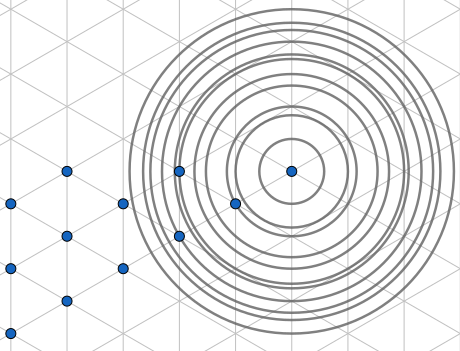
\includegraphics[width=10cm]{challenges/assets/883/illustration_1.png}
    \caption{Example of all possible inner circles for \(r \leq 2.5\), derived from the blue dots that represent a corner with a 60\textdegree angle.}
\end{figure}

Reasoning from the above illustration, we can see that the number of possible radii for a given $r$ is determined by the amount of blue dots that are at most $2r$ distance from the center of the inner circle.
Is we know the position of all (unique) possible blue dots, we know all possible inner inradii.

By finding a formula for all the possible blue dots, we can find a formula for the number of possible inradii.
One can show that the set of possible raddii equals
\begin{equation*}
    \bigcup_{i\in\mathbb{N}^{+}} \left\{ \frac{1}{2}\sqrt{i^2 - ik+k^2} : k\in \mathbb{N}, k\leq\frac{i}{2}\right\}
\end{equation*}
Note that if one wants to find a set of all radii smaller than a given $r$, $R_r$, one can prove that
\begin{equation*}
    R_r \subseteq \bigcup_{i=1}^{\frac{1}{2}i\sqrt{3}\leq r} \left\{ \frac{1}{2}\sqrt{i^2 - ik+k^2} : k\in \mathbb{N}, k\leq\frac{i}{2}\right\}
\end{equation*}
